%%%%%%%%%%%%%%%%%%%%%%%%%%%%%%%%%%%%%%%%%
% Beamer Presentation
% LaTeX Template
% Version 1.0 (10/11/12)
%
% This template has been downloaded from:
% http://www.LaTeXTemplates.com
%
% License:
% CC BY-NC-SA 3.0 (http://creativecommons.org/licenses/by-nc-sa/3.0/)
%
%%%%%%%%%%%%%%%%%%%%%%%%%%%%%%%%%%%%%%%%%

%----------------------------------------------------------------------------------------
%	PACKAGES AND THEMES
%----------------------------------------------------------------------------------------

\documentclass{beamer}

\mode<presentation> {

% The Beamer class comes with a number of default slide themes
% which change the colors and layouts of slides. Below this is a list
% of all the themes, uncomment each in turn to see what they look like.

%\usetheme{default}
%\usetheme{AnnArbor}
%\usetheme{Antibes}
%\usetheme{Bergen}
%\usetheme{Berkeley}
%\usetheme{Berlin}
%\usetheme{Boadilla}
%\usetheme{CambridgeUS}
%\usetheme{Copenhagen}
%\usetheme{Darmstadt}
%\usetheme{Dresden}
%\usetheme{Frankfurt}
%\usetheme{Goettingen}
%\usetheme{Hannover}
%\usetheme{Ilmenau}
%\usetheme{JuanLesPins}
%\usetheme{Luebeck}
\usetheme{Madrid}
%\usetheme{Malmoe}
%\usetheme{Marburg}
%\usetheme{Montpellier}
%\usetheme{PaloAlto}
%\usetheme{Pittsburgh}
%\usetheme{Rochester}
%\usetheme{Singapore}
%\usetheme{Szeged}
%\usetheme{Warsaw}

% As well as themes, the Beamer class has a number of color themes
% for any slide theme. Uncomment each of these in turn to see how it
% changes the colors of your current slide theme.

%\usecolortheme{albatross}
%\usecolortheme{beaver}
%\usecolortheme{beetle}
%\usecolortheme{crane}
%\usecolortheme{dolphin}
%\usecolortheme{dove}
%\usecolortheme{fly}
%\usecolortheme{lily}
%\usecolortheme{orchid}
%\usecolortheme{rose}
%\usecolortheme{seagull}
%\usecolortheme{seahorse}
%\usecolortheme{whale}
%\usecolortheme{wolverine}

%\setbeamertemplate{footline} % To remove the footer line in all slides uncomment this line
%\setbeamertemplate{footline}[page number] % To replace the footer line in all slides with a simple slide count uncomment this line

%\setbeamertemplate{navigation symbols}{} % To remove the navigation symbols from the bottom of all slides uncomment this line
}

\usepackage{graphicx} % Allows including images
\usepackage{booktabs} % Allows the use of \toprule, \midrule and \bottomrule in tables

%----------------------------------------------------------------------------------------
%	TITLE PAGE
%----------------------------------------------------------------------------------------

\title[Short title]{Inversion of a model sedimentary basin using Simulated Annealing} % The short title appears at the bottom of every slide, the full title is only on the title page

\author{Jose Luis Silva} % Your name
\institute[UU] % Your institution as it will appear on the bottom of every slide, may be shorthand to save space
{
Uppsala University \\ % Your institution for the title page
\medskip
\textit{jose.silva@physics.uu.se} % Your email address
}
\date{\today} % Date, can be changed to a custom date

\begin{document}

\begin{frame}
\titlepage % Print the title page as the first slide
\end{frame}

\begin{frame}
\frametitle{Overview} % Table of contents slide, comment this block out to remove it
\tableofcontents % Throughout your presentation, if you choose to use \section{} and \subsection{} commands, these will automatically be printed on this slide as an overview of your presentation
\end{frame}

%----------------------------------------------------------------------------------------
%	PRESENTATION SLIDES
%----------------------------------------------------------------------------------------

%------------------------------------------------
\section{First Section} % Sections can be created in order to organize your presentation into discrete blocks, all sections and subsections are automatically printed in the table of contents as an overview of the talk
%------------------------------------------------

\subsection{Introduction} % A subsection can be created just before a set of slides with a common theme to further break down your presentation into chunks

\begin{frame}
\frametitle{Introduction}
According to Nagy, it is possible to \textbf{describe an arbitrary geological configuration in subsurface considering blocks composed of prisms with different dimensions}. 
\newline \newline
The distribution of vertical components associated with the gravitational attraction of a right rectangular prism with density varying with depth following a third order polynomial can be used to find this geological configuration through through the use of a global optimization algorithms.
\end{frame}

%------------------------------------------------

\subsection{Problem} % A subsection can be created just before a set of slides with a common theme to further break down your presentation into chunks

\begin{frame}
\frametitle{Direct Model - Problem}
A sedimentary basin is constituted by a sedimentary and an homogeneous basement. This sedimentary package is discretized by prisms contained in a finite region of space with a mesh in which the top coincides to the Earth's surface The arbitrary interface separating the sedimentary is described as points by the thickness of each of the prisms.
\begin{figure}[t!]
\begin{center}
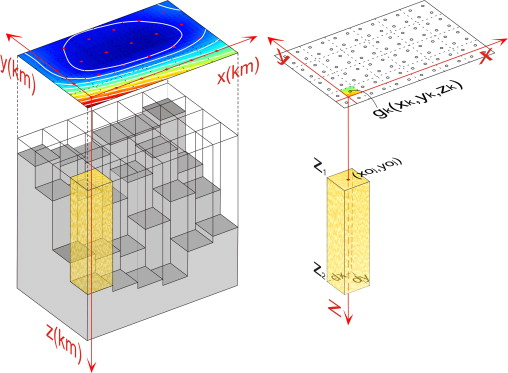
\includegraphics[scale=.6]{./images/prism.png}
\end{center}
\caption{}
\label{fluxo_calor}
\end{figure}
\end{frame}

%------------------------------------------------

\subsection{Gravity anomaly} % A subsection can be created just before a set of slides with a common theme to further break down your presentation into chunks

\begin{frame}
\frametitle{Direct Model}

\begin{itemize}
\item In direct modeling we predict the field generated by a mathematical model and estimate the error with respect to the information obtained in the field.
\end{itemize}
The gravitational attraction of an elementary mass with respect to a unit mass located at a distance $r$ is given by:
\begin{equation}
F_{z} = \int \int \int \frac{G\rho\cos{\gamma} }{{r}^2} dx' dy' dz' 
\end{equation}
Considering a coordinate system with the z-axis schematized according to the figure [citation] where the angle formed between the distance vector $r=\sqrt{(x'-x_0)^2+(y'-y_0)^2+(z'-z_0)^2}$ and the z-axis is given by $ \gamma $. Applying the equation in the differential gravitational attraction component$dF_{z} = dF \cos{\gamma} $, we obtain the following expression:
\end{frame}

%------------------------------------------------

\begin{frame}
\frametitle{Direct Model}
 Applying the equation in the differential gravitational attraction component$dF_{z} = dF \cos{\gamma} $, we obtain the following expression:
 \begin{equation}
F_{z} = \int \int \int \frac{G\rho\cos{\gamma} }{{r}^2} dx' dy' dz' 
\end{equation}
and considering $\cos{\gamma} = (z'-z_0)/r$ :
\begin{eqnarray}
g_z &=& G \int_{x'_1}^{x'_2} \int_{y'_1}^{y'_2} \int_{z'_1}^{z'_2} \frac{\rho(z')\cos{\gamma} }{{r}^3} dx' dy' dz' \nonumber \\ 
&=& G \int_{x'_1}^{x'_2} \int_{y'_1}^{y'_2} \int_{z'_1}^{z'_2} \frac{\rho(z')(z'-z_0)}{ {\left[(x'-x_0)^2+(y'-y_0)^2+(z'-z_0)^2\right]} ^{3/2} } dx' dy' dz'  \nonumber \\
\end{eqnarray}
\end{frame}

%------------------------------------------------

 % A subsection can be created just before a set of slides with a common theme to further break down your presentation into chunks

\begin{frame}
\frametitle{Direct Model}
Applying the following transformation of coordinates:
\begin{eqnarray}
x_n = x'_n - x_0 \\
x_n = y'_n - y_0 \\
z_n = z'_n - z_0 \label{25}
\label{22}
\end{eqnarray}
with n=1,2 in which the prisms are limited by the planes $x'=x'_1,x'_2 ~$, $y'=y'_1.y'_2 ~$ and $z'=z'_1,z'_2$ ; dx'=dx, dy'=dy e dz'=dz, we obtain:
\begin{eqnarray}
g_z= G \int_{x_1}^{x_2}dx \int_{y_1}^{y_2}dy \int_{z_1}^{z_2} \frac{\rho(z')(z'-z_0)dz}{ ({x^2 + y^2 + z^2)} ^{3/2} } \label{26}
\end{eqnarray}
\end{frame}

%------------------------------------------------
\subsection{Direct Model} % A subsection can be created just before a set of slides with a common theme to further break down your presentation into chunks

\begin{frame}
\frametitle{Direct Model}
Considering the following density as a function of the depth as:
\begin{eqnarray}
\rho(z')=p+qz'+rz'^2+sz'^3 
\end{eqnarray}
\begin{eqnarray}
\rho(z) &=& p+q(z+z_0)+r(z+z_0)^2+s(z+z_0)^3 = (p + qz_0 + rz_0^2 + sz_0^3) \nonumber \\ &+& (q + 2rz_0 + 3sz_0^2)z + (r + 3sz_0)z^2 + sz^3 \label{27} \nonumber \\
\end{eqnarray}

Substituting equation (\ref{27}) into (\ref{26}) :

 \begin{eqnarray}
 g_z= G \int_{x_1}^{x_2}dx \int_{y_1}^{y_2}dy \int_{z_1}^{z_2} \frac{(\rho_1 z+\rho_2 z^2+\rho_3 z^3+\rho_4 z^4) dz}{ ({x^2 + y^2 + z^2)} ^{3/2}}  \label{28}
 \end{eqnarray}
\begin{eqnarray}
\rho_1 &=& p + qz_0 + rz_0^2 + sz_0^3 \\
\rho_2 &=& q + 2rz_0 + 3sz_0^2  \\ 
\rho_3 &=& r + 3sz_0 \\
\rho_4 &=& s 
\label{29}
\end{eqnarray}
\end{frame}
%------------------------------------------------

\begin{frame}
\frametitle{Direct Model}
Equation (\ref{28}) can be simplified:
\begin{eqnarray}
 g_z = G\sum_{n=1}^{n=4} \int_{x_1}^{x_2}dx \int_{y_1}^{y_2}dy \int_{z_1}^{z_2} \frac{(\rho_k z^k) dz}{ ({x^2 + y^2 + z^2)} ^{3/2}} =  G\sum_{n=1}^{n=4} I_k   \label{291}
 \end{eqnarray}
 for k=1:
  \begin{eqnarray}
 I_1 = - \rho_1 \int_{x_1}^{x_2}dx \int_{y_1}^{y_2} \frac{1} {({x^2 + y^2 + z^2)} ^{1/2}}dy |_{z_1}^{z_2} = \nonumber \\ 
 - \rho_1 \int_{x_1}^{x_2} {\ln {(y+ \sqrt{{x^2 + y^2 + z^2}})}} dx |_{y_1}^{y_2}|_{z_1}^{z_2} \nonumber \\  \label{i1}
 \end{eqnarray}

\end{frame}

%------------------------------------------------
 % A subsection can be created just before a set of slides with a common theme to further break down your presentation into chunks

\begin{frame}
\frametitle{Direct Model}
Integration $\int fdg = fg - \int g df$ in the equation (\ref{i1}) as dg=dx :

\begin{eqnarray}
&&I_1= -\rho_1 [ x{\ln {(y+ \sqrt{{x^2 + y^2 + z^2}})}}|_{x_1}^{x_2} \nonumber \\ 
&& - \int_{x_1}^{x_2} \frac{x^2{(\sqrt{{x^2 + y^2 + z^2}}-y)}} {(x^2+z^2) \sqrt{x^2 + y^2 + z^2}}dx ]|_{y_1}^{y_2}|_{z_1}^{z_2} \nonumber \\ 
&&= -\rho_1 [ x{\ln {(y+ \sqrt{{x^2 + y^2 + z^2}})}}|_{x_1}^{x_2}  - \int_{x_1}^{x_2} \frac{x^2}{x^2+z^2} dx \nonumber \\ 
&&+ y \int_{x_1}^{x_2} \frac{x^2}{{(x^2+z^2) \sqrt{x^2 + y^2 + z^2}}} ]|_{y_1}^{y_2}|_{z_1}^{z_2} \nonumber \\
\label{i2}
\end{eqnarray}

\end{frame}
%------------------------------------------------
% A subsection can be created just before a set of slides with a common theme to further break down your presentation into chunks

\begin{frame}
\frametitle{Direct Model}
But the second term of the previous equation is 0, which means:
  \begin{eqnarray}
  && I_1 = -\rho_1 [ x{\ln {(y+ \sqrt{{x^2 + y^2 + z^2}})}} \nonumber \\ 
  &&+ y [ \int_{x_1}^{x_2} \frac{x^2+z^2 - z^2}{{(x^2+z^2) \sqrt{x^2 + y^2 + z^2}}} ]]|_{y_1}^{y_2}|_{z_1}^{z_2}  \nonumber \\
  && = -\rho_1 \left[ x{\ln {(y+ \sqrt{{x^2 + y^2 + z^2}})}}|_{x_1}^{x_2}  + I  \right]|_{y_1}^{y_2}|_{z_1}^{z_2} \nonumber \\
  \label{i3}
  \end{eqnarray}  
\begin{eqnarray}
I &=& y  \int_{x_1}^{x_2} \frac{dx}{\sqrt{x^2 + y^2 + z^2}} - yz^2 \int_{x_1}^{x_2} \frac{dx}{{(x^2+z^2) \sqrt{x^2 + y^2 + z^2}}} \nonumber \\ &=& y \left[ {\ln {(x+ \sqrt{{x^2 + y^2 + z^2}})}}|_{x_1}^{x_2}  - z^2 \int_{x_1}^{x_2} \frac{dx}{{(x^2+z^2) \sqrt{x^2 + y^2 + z^2}}}  \right] \nonumber \\
&=& y [ {\ln {(x+ \sqrt{{x^2 + y^2 + z^2}})}} - \frac{z}{y} \arctan{\left(\frac{xy}{z\sqrt{x^2 + y^2 + z^2}}\right)} ]|_{x_1}^{x_2}
\end{eqnarray}

\end{frame}
%------------------------------------------------
% A subsection can be created just before a set of slides with a common theme to further break down your presentation into chunks

\begin{frame}
\frametitle{Direct Model}
Considering $x=\tan{\theta}\sqrt{y^2+z^2}$ and $y \sin{\theta}=\rho$ we can compute $I_1$ through 24 terms after substituting the intergration limits:

\begin{eqnarray}
&& I_1 = \rho_1 (- x{\ln {(y+ \sqrt{{x^2 + y^2 + z^2}})}}- y{\ln {(x+ \sqrt{{x^2 + y^2 + z^2}})}} \nonumber \\ 
 && + z\arctan{\left(\frac{xy}{z\sqrt{x^2 + y^2 + z^2}}\right)} )  |_{x_1}^{x_2}|_{y_1}^{y_2}|_{z_1}^{z_2} \nonumber \\
\end{eqnarray}
This solution is applied to problems whose prisms exhibits a constant density ($\rho_1 = cte, \rho_2=rho_3=\rho_4=0$).  \textbf{Our model is based on the density as a cubic polynomial equation}, which guides us towards the recurrence formulas for $I_2,I_3$ e $I_4$.
\end{frame}
%------------------------------------------------
\subsection{I for k=2} % A subsection can be created just before a set of slides with a common theme to further break down your presentation into chunks

\begin{frame}
\frametitle{Direct Model}
For k=2:
 \begin{eqnarray}
&&I_2 =  \rho_2 \int_{x_1}^{x_2}dx \int_{y_1}^{y_2} dy \int_{z_1}^{z_2} \frac{z^2 dz} {({x^2 + y^2 + z^2)} ^{3/2}} \nonumber \\   
&&= \rho_2 \int_{x_1}^{x_2}dx \int_{y_1}^{y_2} dy \left[ {\ln {(z+r)} - \frac{z}{r}}  \right]  |_{z_1}^{z_2} \nonumber \\  
&&= \rho_2 \int_{x_1}^{x_2}dx \left[ {y\ln {(z+r)} - x\arctan{\left(\frac{zy}{xr}\right)}}  \right]|_{y_1}^{y_2}|_{z_1}^{z_2} \nonumber \\
&&= \rho_2 [ yx\ln{(z+r)}-\frac{y^2}{2}\arctan{\left(\frac{zx}{yr}\right)} - \frac{x^2}{2}\arctan{\left(\frac{zy}{xr}\right)} \nonumber \\  
&&+ \frac{z^2}{2}\arctan{\left(\frac{xy}{zr}\right)} ]|_{x_1}^{x_2}|_{y_1}^{y_2}|_{z_1}^{z_2} \nonumber \\
 \label{i11}
\end{eqnarray}
\end{frame}
%------------------------------------------------
\subsection{I for k=3} % A subsection can be created just before a set of slides with a common theme to further break down your presentation into chunks

\begin{frame}
\frametitle{Direct Model}
For k=3:
 \begin{eqnarray}
&&I_3 =  \rho_3 \int_{x_1}^{x_2}dx \int_{y_1}^{y_2} dy \int_{z_1}^{z_2} \frac{z^3 dz} {{(x^2 + y^2 + z^2)} ^{3/2}} \nonumber \\ 
&&= \rho_3 \int_{x_1}^{x_2}dx \int_{y_1}^{y_2} dy \left[ {r + \frac{(x^2+y^2)}{r}}  \right]  |_{z_1}^{z_2} \nonumber \\  
&&= \rho_3 \int_{x_1}^{x_2}dx \left[ {x^2\ln {(y+r)} + yr}  \right]|_{y_1}^{y_2}|_{z_1}^{z_2} \nonumber \\
&&= \rho_3 \left[ \frac{y^3}{3}\ln{(x+r)}+\frac{x^3}{3}\ln{(y+r)}+\frac{z^3}{3}\arctan{\left(\frac{xy}{zr}\right)}-\frac{2}{3} xyr \right]|_{x_1}^{x_2}|_{y_1}^{y_2}|_{z_1}^{z_2} \nonumber \\
 \label{i12}
 \end{eqnarray}
\end{frame}
%------------------------------------------------
\subsection{I for k=4}
\begin{frame}
\frametitle{Direct Model}
For k=4:
\begin{eqnarray}
&&I_4 =  \rho_4 \int_{x_1}^{x_2}dx \int_{y_1}^{y_2} dy \int_{z_1}^{z_2} \frac{z^4 dz} {{(x^2 + y^2 + z^2)} ^{3/2}} \nonumber \\
&& = \rho_4 \int_{x_1}^{x_2}dx \int_{y_1}^{y_2} dy \left[ {\frac{1}{2}zr + \frac{(x^2+y^2)}{r}z - \frac{3}{2}(x^2+y^2)\ln{(z+r)}} \right]  |_{z_1}^{z_2} \nonumber \\  
&&= \rho_4 \int_{x_1}^{x_2}dx [{\frac{1}{2}yzr + x^3\arctan{\left(\frac{yz}{xr}\right)}  - \frac{1}{2}y^3 \ln{(z+r)} - \frac{3}{2}x^2 y \ln{(z+r)}}]|_{y_1}^{y_2}|_{z_1}^{z_2} \nonumber \\
&&= \rho_4 [ \frac{z^4}{4}\arctan{\left(\frac{xy}{zr}\right)}+\frac{x^4}{4}\arctan{\left(\frac{yz}{xr}\right)} + \frac{y^4}{4}\arctan{\left(\frac{zx}{yr}\right)} \nonumber \\
&& -\frac{xy}{2}(x^2+y^2)\ln{(z+r)} -\frac{xyzr}{4} ]|_{x_1}^{x_2}|_{y_1}^{y_2}|_{z_1}^{z_2} \nonumber \\
\label{i13}
\end{eqnarray}
\end{frame}
%------------------------------------------------
\subsection{Direct model parameters}
\begin{frame}
\frametitle{Direct Model - Basalt Prism }
\begin{figure}[t!]
\begin{center}
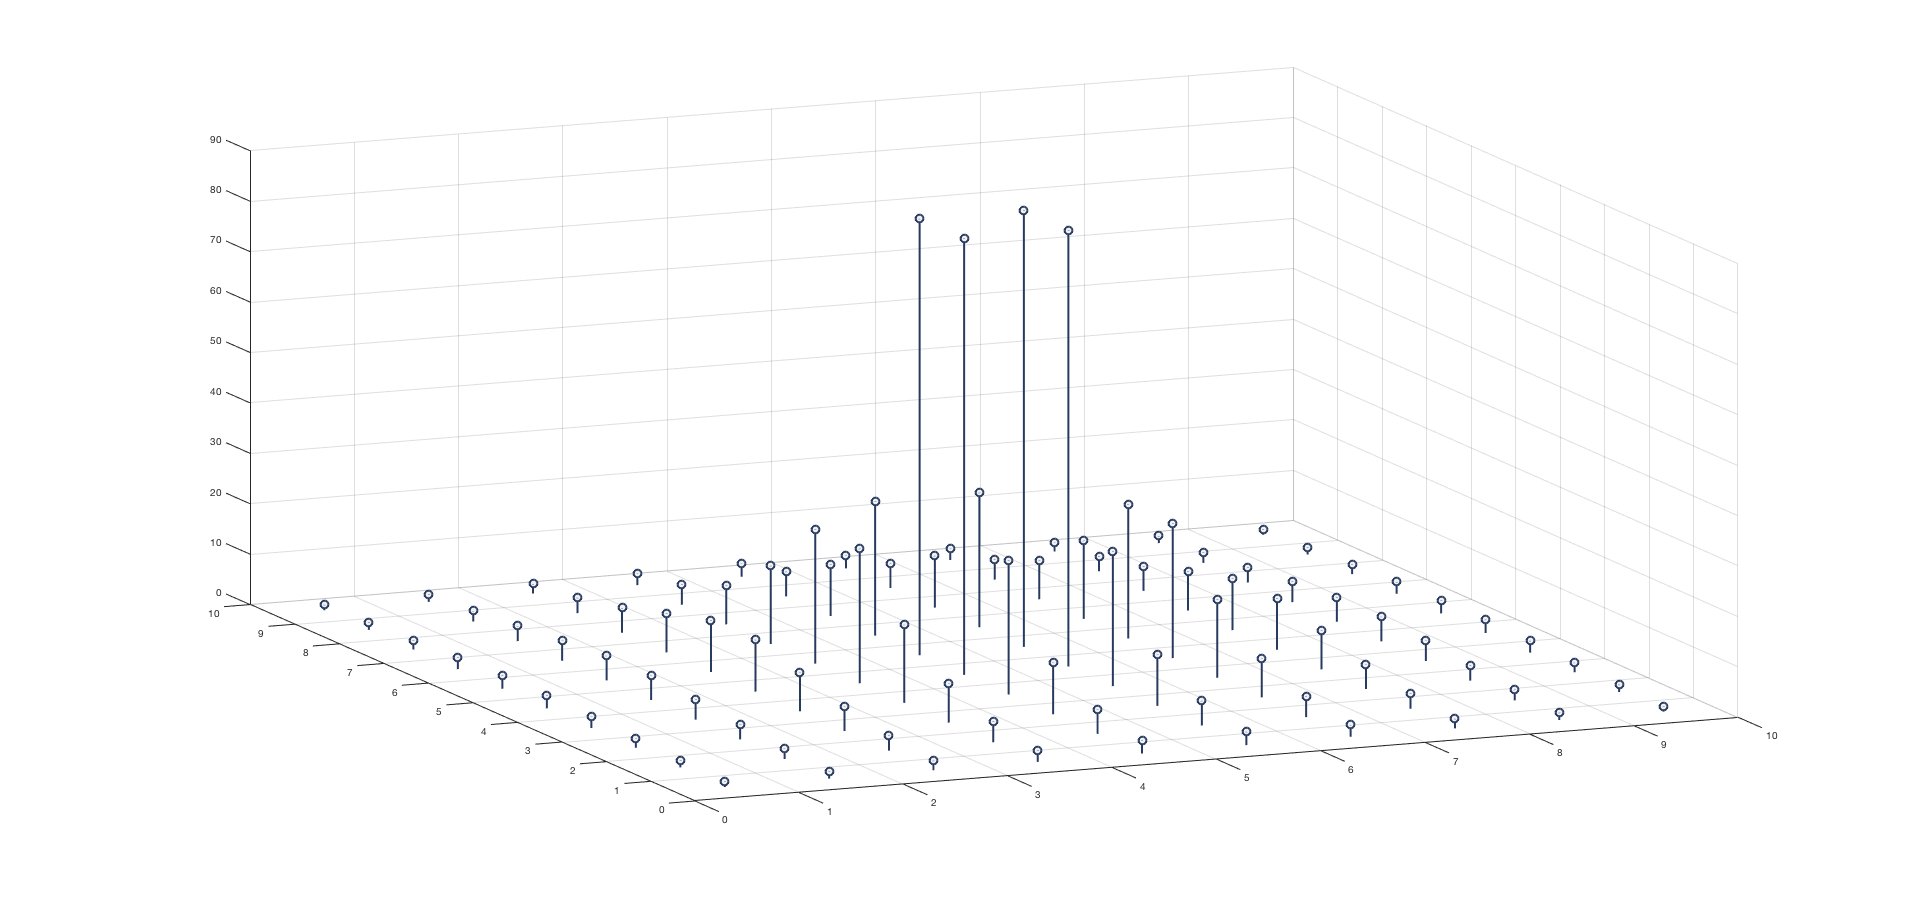
\includegraphics[scale=.15]{./images/grid10.png}
\end{center}
\caption{ Rectangular Prism : $x_1=4$,$y_1=4$,$z_1=0$,$x_2=6$,$y_2=6$,$z_1=3$ $p_1=2560$,$q_1=0$,$r_1=0$,$s_1=0$, grid from 0 until 10 km.}
\label{fluxo_calor}
\end{figure}
\end{frame}
%------------------------------------------------
\begin{frame}
\frametitle{Direct Model - Prism 40x40x60x60x3}
\begin{figure}[t!]
\begin{center}
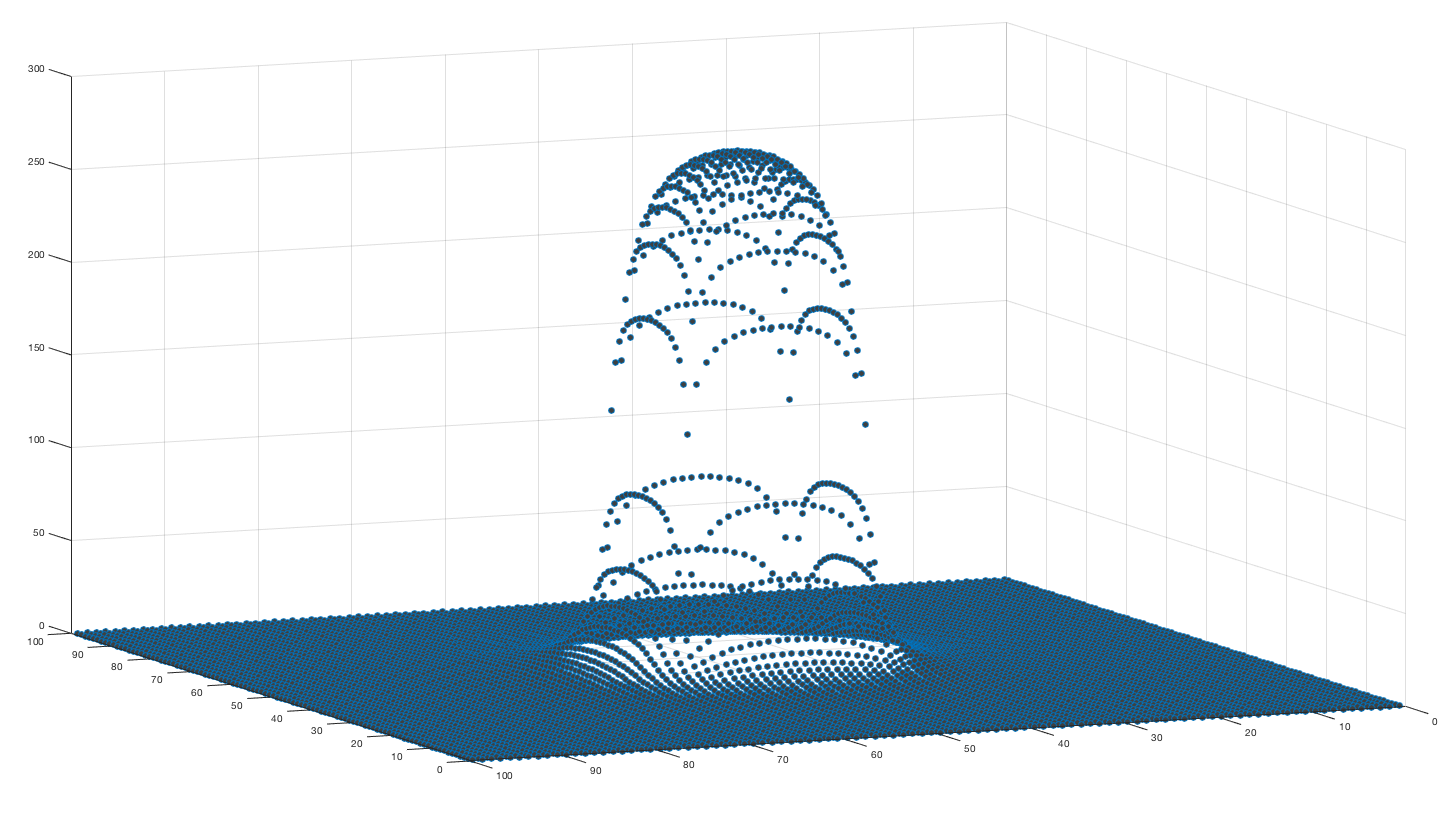
\includegraphics[scale=.20]{./images/gri100x100.png}
\end{center}
\caption{.}
\label{fluxo_calor}
\end{figure}
\end{frame}
%------------------------------------------------
\begin{frame}
\frametitle{Inversion - SA Algorithm}

\begin{itemize}
\item How to solve this problem using optimization algorithms?
\begin{block}{Evolutionary Algorithms}
The simulated annealing method simulates the process of slow cooling of molten
metal to achieve the minimum function value in a minimization problem. The cooling
phenomenon of the molten metal is simulated by introducing a temperature-like parameter
and controlling it using the concept of Boltzmann’s probability distribution.
\end{block}
\end{itemize}
Boltzmann’s probability distribution implies that the energy (E) of a system in thermal
equilibrium at temperature T is distributed probabilistically according to:
\begin{eqnarray}
P(E)=exp(\frac{E} {k_b T})
\end{eqnarray}
\end{frame}
%------------------------------------------------
\section{Second Section}
%------------------------------------------------
\begin{frame}
\frametitle{Inversion - SA Algorithm}

\begin{itemize}
\item The convergence of the simulated annealing algorithm can be controlled by controlling the
temperature T.
\item Start with an initial design vector
X1 (iteration number i = 1) and a high value of temperature T . 
\item Generate a new design point randomly in the vicinity of the current design point and find the difference in
function values:  $\Delta{E}=E_{i+1} - E_{i} = f_{X_{i+1}}-f_{X_{i}}$
\item If $\Delta{E}\leq 0$ than $P[E_{i+1}]=1$ and ${X_{i+1}}$ is accepted
\item If $\Delta{E} > 0$ then the probability of accepting
the point $X_{i+1}$, in spite of its being worse than $X_i$ in terms of the objective function
value, is finite (although it may be small) according to the Metropolis criterion.
\end{itemize}
\end{frame}
%------------------------------------------------
\begin{frame}
\frametitle{Inversion - SA Algorithm}

\begin{itemize}
\begin{block}{Metropolis criterion}
According to Metropolis criterion, the probability of the next design point
(state) $X_{i+1}$ depends on the difference in the energy state or function values at the two
design points (states).  $P[E_{i+1}]=[exp(\frac{\Delta E} {T})]$
\end{block}
\item If the temperature T is large, the probability will be high
for design points $X_{i+1}$ with larger function values, even worse design can be accepted.
\item if the temperature T is small, the probability
of accepting worse design points $X_{i+1}$
\item as the temperature values get smaller the  process gets closer to the
optimum solution.
\end{itemize}
\end{frame}
%------------------------------------------------
\subsection{SA code} % A subsection can be created just before a set of slides with a common theme to further break down your presentation into chunks

\begin{frame}
\frametitle{Code}
\begin{itemize}
\item Generate z and density: \\
$z_n(i,j) = REAL(z(i,j) + 2*e*z(i,j)*(ran3(idum) - 0.5)) $ \\
$p_n = REAL(p1 + 2*e*p1*(ran3(idum) - 0.5))$
$q_n = REAL(q1 + 2*e*q1*(ran3(idum) - 0.5))$
$r_n = REAL(r1 + 2*e*r1*(ran3(idum) - 0.5))  $
$s_n = REAL(s1 + 2*e*s1*(ran3(idum) - 0.5)) $
\item Metropolis : \\
$IF (fx_n < fx) $THEN - accept \\
ELSE  $IF ((EXP(-(fx_n - fx)/temperatura) > ran3(idum)) .and. (naccepted < a)  )$ THEN - accept \\
\item Temperature decay:\\
$temperatura = temperatura * tfactor$\\
\item Heating process:\\
$IF ((temperatura < 0.001).and.(emin > 0.1)) $ THEN \\
$temperatura = 7.0$ \\
END IF
\end{itemize}
\end{frame}

%------------------------------------------------
\subsection{Results}
\begin{frame}
\frametitle{Parameters to start the optimization: \\}

\begin{block}{Parameters}
 $p_1$ =    2000.0000000000000  ;   $q_1$ =    100.00000000000000     \\
 $r_1$ =    100.00000000000000   ;   $s_1$ =    1000.0000000000000     \\
 $z_0$ =    0.0000000000000000   ;   $z_1$ =    0.0000000000000000     \\
 $xmin$ =    0.0000000000000000   ;    xmax =    10.000000000000000     \\
 $ymin$ =    0.0000000000000000   ;    ymax =    10.000000000000000     \\
 temperature =   8.0000000000000000    ;  tfactor =  0.4000000000000000  \\
 nsteps =        1000   ;  idum =  10 ;  istep =    1  ;  jstep =  1    \\
 FINISH-start   880.25350200000003 seconds   \\   
 Solution:
$p_1$ =    2562.0402832031250  ; $q_1$ =    5.3528009448200464E-004    \\ 
$r_1$ =    1.8700489774346352E-002   ; $s_1$ =    8.7235484897973947E-006 \\
Cost function: 3.4913883283133424
\end{block}
\end{frame}

%------------------------------------------------

\begin{frame}
\frametitle{Temperature x Cost function}
\begin{figure}[t!]
\begin{center}
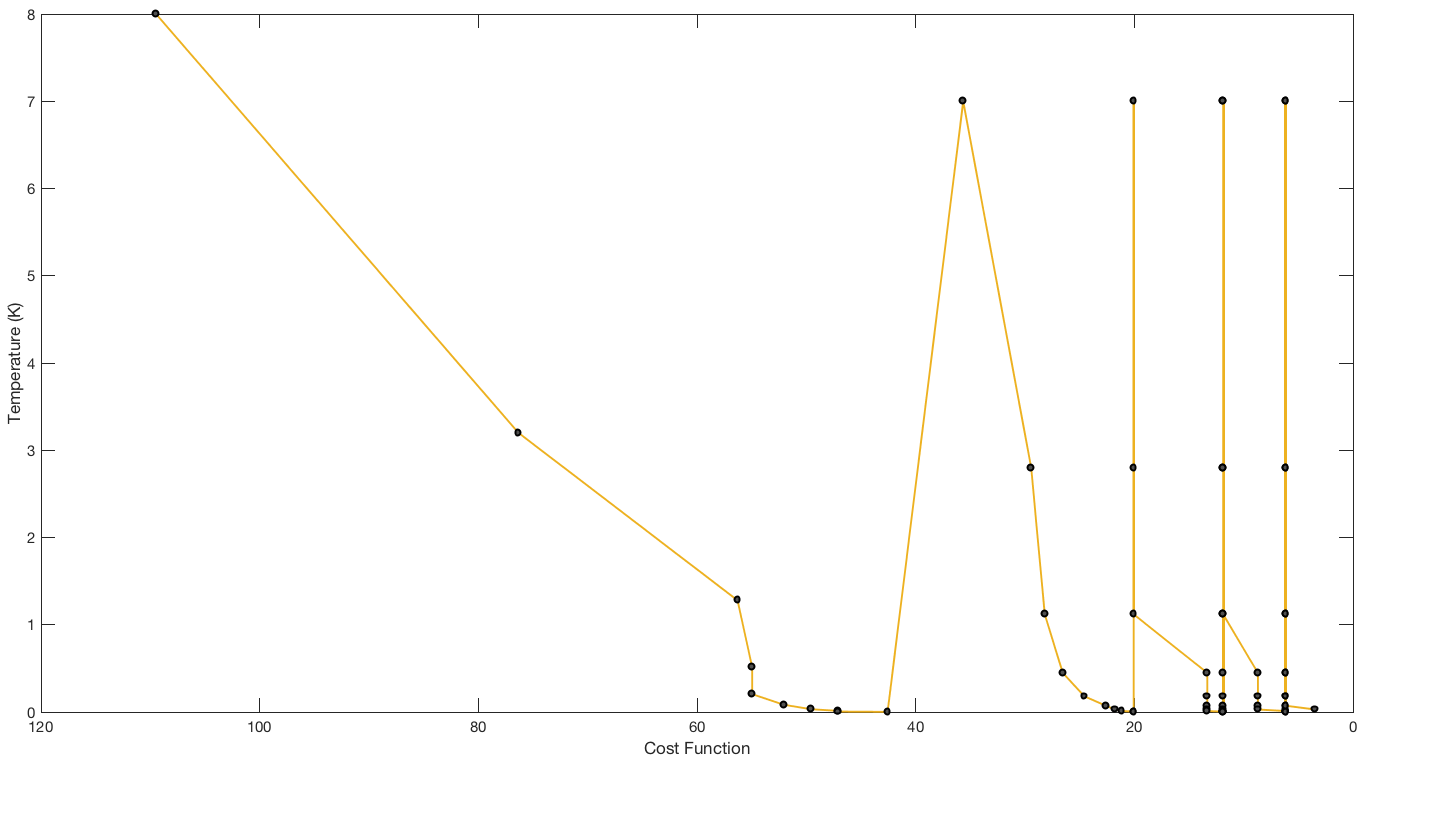
\includegraphics[scale=.25]{./images/COST_TEMP.png}
\end{center}
\caption{Final steps after termalization}
\label{fluxo_calor}
\end{figure}
\end{frame}
%------------------------------------------------
\begin{frame}
\frametitle{Temperature x Cost function}
\begin{figure}[t!]
\begin{center}
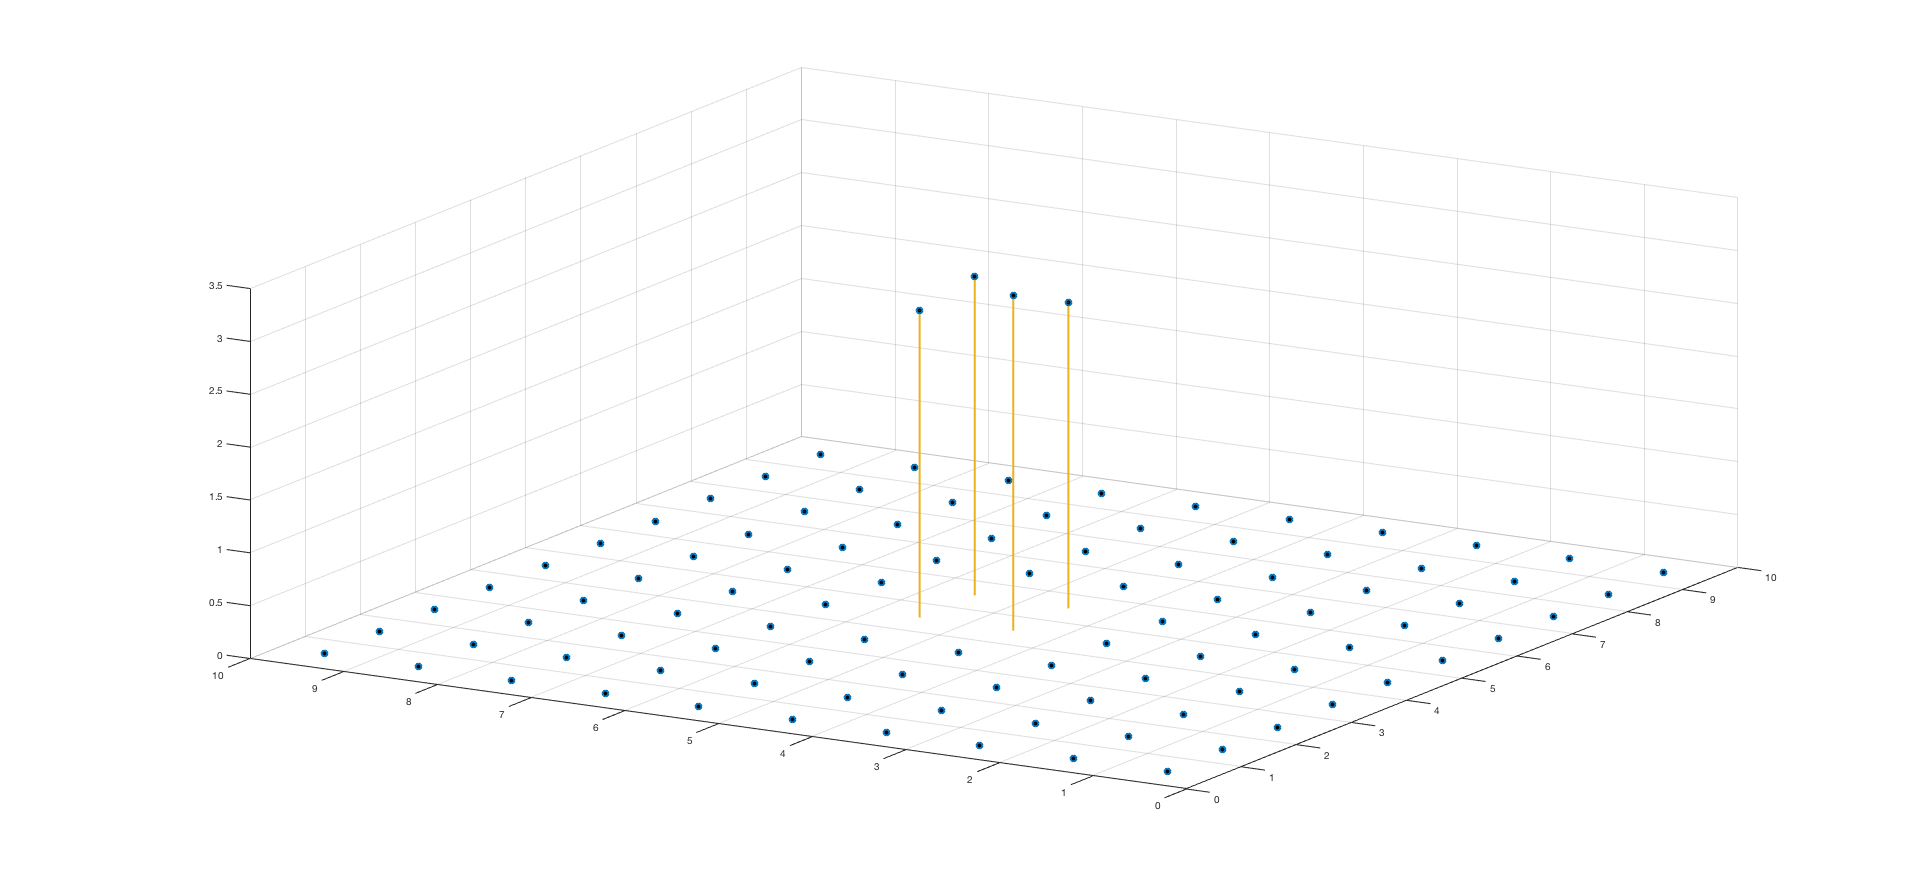
\includegraphics[scale=.17]{./images/inversion.png}
\end{center}
\caption{Prediction of the subsurface after 14 min with an error < $10^-3$ due to the chosen cutoff of 3 for the cost function.}
\label{fluxo_calor}
\end{figure}
\end{frame}
%------------------------------------------------

\subsection{References}
\begin{frame}
\frametitle{References}
\footnotesize{
\begin{thebibliography}{99} % Beamer does not support BibTeX so references must be inserted manually as below
\bibitem[Juan Garcia Abdeslem 2005]{p1} Garcia (2005)
\newblock  The gravitational attraction of a right rectangular prism with density varying with depth following a cubic polynomial” GEOPHYSICS, 31(2), 362-371.
\end{thebibliography}
\begin{thebibliography}{99} % Beamer does not support BibTeX so references must be inserted manually as below
\bibitem[Richard J. Blakely  1996]{p1} Blakely (1996)
\newblock  Potential Theory in Gravity and Magnetic Applications” United States Geological Survey.
\end{thebibliography}
\begin{thebibliography}{99} % Beamer does not support BibTeX so references must be inserted manually as below
\bibitem[Dezsö Nagy 1966]{p1} Nagy (1966)
\newblock  THE GRAVITATIONAL ATTRACTION OF A RIGHT RECTANGULAR PRISM.” GEOPHYSICS, 31(2), 362-371.
\newblock \emph{GEOPHYSICS} 31(2), 362-371.
\end{thebibliography}
}
\end{frame}

%------------------------------------------------

\begin{frame}
\Huge{\centerline{The End}}
\end{frame}

%----------------------------------------------------------------------------------------

\end{document}